\begin{frame}
  \frametitle{Application to D.~D.\ Convection}
  \begin{itemize}
    \item{ We now proceed to use the flux formula to
      compute Sherwood numbers for the double-diffusion problem
      \vspace{-.2in}
      \begin{center}
	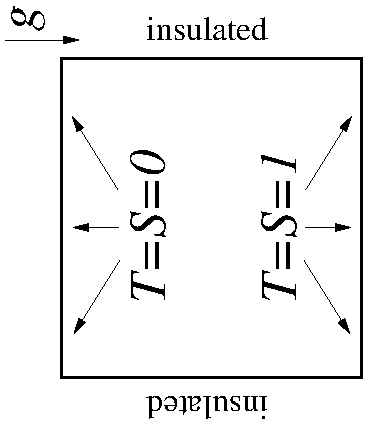
\includegraphics[width=.3\textwidth,angle=-90]{figures/setup}
      \end{center}
    }
    \item{The goal is to compute the steady state value of 
      $I := -\int\nabla S \cdot n \;dx$ or $-\int\nabla T \cdot n \;dx$
      at the bottom (or top) of the enclosure.}
  \end{itemize}
\end{frame}



\begin{frame}
  \frametitle{Application to D.~D.\ Convection}
  \begin{itemize}
    \item{As a simple test problem, we consider the case $\kappa=1$.}
    \item{In this case, $T=S$ at steady state so it suffices to consider
      the flux of only a single variable. }
  \end{itemize}
\end{frame}

\begin{frame}
  \frametitle{Application to D.~D.\ Convection}
    \vspace{-.25in}
    \begin{center}
	\includegraphics[width=.8\textwidth]{figures/kappa1_solute_error_bilinears.pdf}    
  \end{center}
    \vspace{-.2in}
    \begin{itemize}
      \item{Surprisingly, the classical method is actually \emph{better} here.}
    \end{itemize}
\end{frame}

\begin{frame}
  \frametitle{Application to D.~D.\ Convection}\vspace{-.25in}
    \begin{center}
	\includegraphics[width=.8\textwidth]{figures/kappa1_solute_error_biquadratics.pdf}    
  \end{center}
\vspace{-.2in}
    \begin{itemize}
      \item{For biquadratics, the boundary flux formula recovers the $p+1$ rate.}
    \end{itemize}
\end{frame}
